\documentclass[12pt]{article}
\usepackage{fullpage}
\usepackage{titlesec}
\usepackage{tikz}
\usepackage{amsfonts,amssymb}
\usepackage{amsmath}
\usepackage{comment}
\usetikzlibrary{automata, positioning}

\input ../libraries/mac.tex
\input ../libraries/mathmac.tex

\begin{document}
\pagestyle{plain}
\titleformat{\subsection}[runin]
  {\normalfont\large\bfseries}{\thesubsection}{1em}{}

\title{Homework 4}
\author{Brooke Fugate, Michael O'Connor, Rohan Shah}
\date{}

\maketitle

\section*{Problem B5}
\subsection*{(a)}
Let $M = (K, \Sigma, \Delta, \lambda, q_0, F)$ be an $a$-transducer where
$K = F = \{q_0\}$, $\Sigma = \Delta = \{a,b\}$ and we can define $\lambda$
by induction over the words $u\in \Sigma^*$ and $v \in \Delta^*$ such that
$(q_0, \epsilon, \epsilon, q_0) \in \lambda$ is the base case and by induction
if $(q_0, u, v, q_0) \in \lambda$ then $(q_0,au,bv,q_0), (q_0,bu,av,q_0) \in
\lambda$. A figure that illustrates the $a$-transducer $M$ is:
\begin{center}
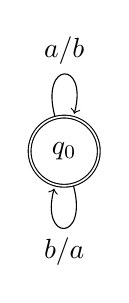
\begin{tikzpicture}[shorten >=1pt, node distance=2.5cm, on grid, auto]
  \node[state, accepting] (q0) {$q_0$};
  \path[->]
(q0) edge [loop above] node {$a/b$} (q0)
(q0) edge [loop below] node {$b/a$} (q0)
  ;
\end{tikzpicture}
\end{center}

\subsection*{(b)}
To prove that the language $R$ is regular we will construct an NFA $N$ using
the given $a$-transducer $M = (K, \Sigma, \Delta, \lambda, q_0, F)$ and alphabet
$T = \{[p,u,v,q] \mid (p,u,v,q) \in \lambda\}$ and prove that $L(N) = R$ thereby
proving $R$ is regular by NFA construction. Let $N = (K, T, \delta, q_0, F)$
where $\delta$ is defined such that
$$\forall p \in K,\ \delta(p, [p,u,v,q]) = q \iff [p,u,v,q] \in \lambda$$
We also define the language $R'$ such that $R \subseteq R'$ where
$$R' = \{[q_o, u_1,v_1,q_1] \cdots [q_{m-1},u_m,v_m,q_m] \mid
[q_{i-1},u_i,v_i,q_i] \in T, 1 \le i \le m, m \ge 1\} \cup \{\epsilon\}$$
and the function $\sigma : T^* \rightarrow K$ such that
$$\sigma(\epsilon) = q_0$$
$$\forall a \in T^* \text{ where }
a = a'[p,u,v,q],\ \sigma(a) = \sigma(a'[p,u,v,q]) = q$$
\textbf{Claim: } $\forall a \in T^*,\ \delta^*(q_0, a) = q \iff a \in R'
\text{ and } \sigma(a) = q$
\newline
\textbf{Proof: } By induction on the length of $a$.
\newline
Base Case: $|a| = 0$ therefore $a = \epsilon$.
$$\delta^*(q_0, \epsilon) = q_0 = \sigma(\epsilon) \text{ and }\epsilon \in R'$$
Inductive Case: $|a| = n+1$ therefore $a = a'[p,u,v,q]$ such that $a,a' \in T^*$
and $|a'| = n$.
Induction Hypothesis: $\delta^*(q_0, a') = p \implies a' \in R' \text{ and }
\sigma(a') = p$
$$ \delta^*(q_0, a) = \delta^*(q_0, a'[p,u,v,q]) =
\delta(\delta^*(q_0, a') ,[p,u,v,q]) = \delta(p, [p,u,v,q) = q$$
$$\sigma(a) = \sigma(a'[p,u,v,q]) = q$$
$$a' \in R \implies a'b \in R,\ \forall b \in T \implies a'[p,u,v,q] \in R
\implies a \in R$$
Since we know that $R \subseteq R'$ we can use the above claim to rewrite the
language $R$ as $$R = \{a \in R' \mid \sigma(a) \in F\}$$
We can now finish our proof by proving that $L(N) = R$.
$$L(N) = \{a \in T^* \mid \delta^*(q_0, a) \in F\}$$
$$\delta^*(q_0, a) \in F \iff \sigma(a) \in F \text{ and } a \in R'
\text{ (by the above claim)}$$
$$L(N) = \{a \in R' \mid \sigma(a) \in F\} = R$$
Therefore, since the NFA $N$ defines the language, $R$ is regular.

\subsection*{(c)}
Given the homomorphism $f : T^* \rightarrow \Sigma^*$ we can define the inverse
image of the language $L \subseteq \Sigma^*$ as
$$f^{-1}(L) = \{a \in T^* \mid f(a) \in L)$$
And we know that $a\in T^*$ implies that $a = a_1a_2 \cdots a_n$ such that
$a_i \in T$, $n \ge 0$, and $a_i = [p_i, u_i, v_i, q_i]$.
We also know that $f([p,u,v,q]) = u$ by the definition of our homomorphism so
$$f(a) = f(a_1a_2\cdots a_n) = f(a_1)f(a_2)\cdots f(a_n) = u_1u_2\cdots u_n$$
Therefore we can rewrite the inverse image of $L$ as
$$f^{-1}(L) =
\{[p_1,u_1,v_1,q_1][p_2,u_2,v_2,q_2]\cdots [p_n,u_n,v_n,q_n] \in T^*$$
$$\mid [p_i,u_i,v_i,q_i] \in T,\ u_1u_2\cdots u_n \in L,\ n \ge 1\} \cup
\{\epsilon \mid \epsilon \in L\}$$
and by definition we have
$$ R = \{[q_0, u_1, v_1, q_1][q_1, u_2, v_2, q_2]\cdots
[q_{n-2}, u_{n-1}, v_{n-1}, q_{n-1}][q_{n-1}, u_n, v_n, q_n]$$
$$\mid  [q_{i-1}, u_i, v_i, q_i]\in T,\, q_n\in F,\, n\geq 1\}
\cup \{\epsilon\ |\ q_0\in F\}$$
thus we have
$$f^{-1}(L)\cap R  = \{[q_0, u_1, v_1, q_1][q_1, u_2, v_2, q_2]\cdots
[q_{n-2}, u_{n-1}, v_{n-1}, q_{n-1}][q_{n-1}, u_n, v_n, q_n]$$
$$ \mid  [q_{i-1}, u_i, v_i, q_i]\in T,\, u_1u_2\cdots u_n\in L,\,
q_n\in F,\, n\geq 1\}\cup \{\epsilon\ |\ q_0\in F,\, \epsilon\in L\}$$
which is what we are trying to prove.

\subsection*{(d)}
Given the homomorpism $g : T^* \rightarrow \Delta$ we can define the image of
the language $f^{-1}(L)\cap R\subseteq T^*$ as
$$g(f^{-1}(L)\cap R) = \{g(a) \mid a \in f^{-1}(L)\cap R\}$$
and we know that $a \in f^{-1}(L)\cap R$ implies that $$a =
[q_0, u_1, v_1, q_1][q_1, u_2, v_2, q_2]\cdots
[q_{n-2}, u_{n-1}, v_{n-1}, q_{n-1}][q_{n-1}, u_n, v_n, q_n]$$ such that
$[q_{i-1}, u_i, v_i, q_i]\in T$, $u_1u_2\cdots u_n\in L$, $q_n\in F$ and
$n\geq 1$. And by the construction of $T$ we have that if $[p,u,v,q] \in T$
then $(p,u,v,q) \in \lambda$. By the definition of an $a$-transducer we have
that if $(p,u,v,q) \in \lambda$ then $(p, u\alpha, \beta) \vdash_M (q,a,\beta v)$
and by transitive and reflexive closure
$(p,w, \epsilon) \vdash_M^* (q,\epsilon,y)$ for some $w \in \Sigma^*$ and
$y \in \Delta^*$. Therefore $a \in f^{-1}(L)\cap R$ implies
$(q_0,w,\epsilon) \vdash_M^* (q_n, \epsilon, y)$ such that $q_n \in F$.
And, since $g([p,u,v,q]) = v$ we have $g(a) = v_1v_2\cdots v_n \in \Delta^*$ by
a similar proof to the one briefly described for $f(a)$ in the previous part.
So we can rewrite the image of $f^{-1}(L)\cap R$ as
$$g(f^{-1}(L)\cap R) = \bigcup _{w\in L} \{y \in \Delta^*
\mid (q_0, w, \epsilon) \vdash_M^* (q_n, \epsilon, y),\ q_n \in F\} =
\bigcup _{w\in L} M(w) = M(L)$$
which is what we wanted to prove. We can also show that $\s{L}$ is closed under
$a$-transduction. We have $f^{-1}(L) \in \s{L}$ by the fact that $\s{L}$ is
closed under inverse homomorphic images. Since we proved that $R$ is regular we
also have that $f^{-1}(L) \cap R \in \s{L}$ by the fact that $\s{L}$ is closed
under intersection with regular languages. Finally we have that
$g(f^{-1}(L) \cap R) \in \s{L}$ by the fact that $\s{L}$ is closed under
homomorphic images. And we just proved that $g(f^{-1}(L) \cap R) = M(L)$ so we
have $M(L) \in \s{L}$ which means $\s{L}$ is closed under $a$-transduction.
Finally we can prove that if $L$ is regular then $M(L)$ regular. Since $L$ is
regular, and the regular languages are closed under intersection, homomorphism,
and inverse homomorphism, we know that $g(f^{-1}(L) \cap R) = M(L)$ is regular.

\subsection*{(e)}
We can define an $a$-transducer, $M_2 = (K, \Delta,\Sigma,\lambda_2,q_0, F)$
such that $(q,v,u,p) \in \lambda_2 \iff (p,u,v,q) \in \lambda$. It is clear then
that $L(M_2) = M^{-1}(L')$ where
$$M^{-1}(L') = \bigcup _{y\in L'} M^{-1}(y)
= \bigcup _{y\in L} \{w \in \Sigma^* \mid y \in M(w)\}$$
$$ = \bigcup _{y\in L'} \{w \in \Sigma^*
\mid y \in \{y \in \Delta^*
\mid (q_0, w, \epsilon) \vdash_M^* (f, \epsilon, y),\ f \in F\}\}$$
$$= \{w \in \Sigma^* \mid (q_0, w, \epsilon) \vdash_M^* (f, \epsilon, y)
,\ f\in F, y\in \Delta^*\}$$
Therefore, since the language $M^{-1}(L')$
is defined by an $a$-transducer and we have already proven that regular languages
are closed under $a$-transduction, if $L'$ is regular then $M^{-1}(L')$ is also
regular.
\end{document}
